%% Tesis_umsa.cls
%% Derechos de Autor 2021 Ruddy Quispe Tapia 
%% <ruddyqt@gmail.com>
%%================================================
%  Plantilla LaTeX para la tesis de licenciatura 
%% según la Carrera de  Econnomia de la Universidad
%% Mayor de San Andres U.M.S.A
%==================================================
%% INFORMACIÓN DE TESIS
%% ---------------------
%% Pon aquí el título, el nombre del autor, Mencion, 
%% el tema..
%% Los "Packages" que pretende utilizar los puede cargar 
%% en la Carpeta " Preambulo/packages "
%   

%% -----------------------------------------
\documentclass{Tesis_umsa}
%%%
%% 
% =======================================
%%%%%%%%%%%%%%%%%%%%%%%%%%%%%%%%%%%%%%%%%%
%% Los paquetes que pretende utilizar     %
%%%%%%%%%%%%%%%%%%%%%%%%%%%%%%%%%%%%%%%%%

% PACKAGES 
% ======================
\usepackage{tcolorbox}
\usepackage{calligra}
\usepackage{booktabs}
\usepackage{bbding}

 

%%%%%%%%%
\thesisUniversity{UNIVERSIDAD  MAYOR DE SAN ANDRES}
\thesisFacultad{FACULTAD DE CIENCIAS ECONÓMICAS Y FINANCIERAS}
\thesisCarrera{CARRERA DE ECONOMÍA}
\thesisGrado{TESIS DE GRADO}
\thesisMencion{Mención: Economía Financiera}
\title{" Titulo de la Tesis "}
\author{xxxx xxxxx .}
\tutor{xxxxx xxxxx}
\relator{xxxxx xxxxx} 
\date{2021}

\begin{document}

\maketitle
\begin{Agradecimientos}

\begin{center}

{\fontfamily{calligra}\fontsize{30}{0}\selectfont{A}}
\textit{gradecemos a los  docentes de la Universidad Mayor de San Andres de la Carrera de Economía, por haber compartido sus conocimientos a lo largo de la preparación de nuestra profesión, de manera especial, al Msc. tutor de nuestro proyecto de investigación quien ha guiado con su paciencia, y su rectitud como docente, y a los ................por su valioso aporte para la presente  investigación.}


\end{center}

{\fontfamily{cmdh}\selectfont{Ejemplo}}
\end{Agradecimientos}

%%\rule{15cm}{1pt}
%\begin{center}
%\makebox[0pt][l]{\rule[1.5pt]{3cm}{3pt}}\rule{3cm}{1pt}
%\end{center}
% 
%
%{\color{red}\hrule height 1pt}%  % default height of \hrule is '0.4pt'
%{\color{lightgray}\hrule height 1mm }% replacement for "\kern1mm"
%{\color{green}\hrule}
%
%
% \myRule{1cm}{1cm}
% 
% \myRule[red]{1cm}{3cm}
%
% \myRule[blue]{1cm}{1cm}
%
% \textcolor{blue}{\rule{2cm}{2cm}}

\begin{Dedicatoria}
\begin{center}
{\fontfamily{calligra}\fontsize{25}{0}\selectfont{D}}
\textit{edico esta tesis  A. DIOS, a Santo Tomás de Aquino, patrono de los estudiantes y a la Virgen María, quienes inspiraron mi espíritu para la conclusión de esta tesis. A mis  padres quienes me dieron vida, educación,  apoyo y consejos. A mis compañeros de estudio, a mis maestros y amigos, quienes sin su ayuda nunca hubiera podido hacer esta tesis. A todos ellos se los agradezco desde el fondo de mi alma. Para todos ellos hago esta dedicatoria.}
\end{center}
\end{Dedicatoria}

%%\rule{15cm}{1pt}
%\begin{center}
%\makebox[0pt][l]{\rule[1.5pt]{3cm}{3pt}}\rule{3cm}{1pt}
%\end{center}
% 
%
%{\color{red}\hrule height 1pt}%  % default height of \hrule is '0.4pt'
%{\color{lightgray}\hrule height 1mm }% replacement for "\kern1mm"
%{\color{green}\hrule}
%
%
% \myRule{1cm}{1cm}
% 
% \myRule[red]{1cm}{3cm}
%
% \myRule[blue]{1cm}{1cm}
%
% \textcolor{blue}{\rule{2cm}{2cm}}

\begin{Resumen}
La presente tesis tiene como objetivo general investigar el efecto que genera la Bolivianización, el Índice del tipo de cambio real, la Remesas y las Exportaciones 


%(excluyendo los ingresos por exportación del gas natural) sobre la Fluctuación de las Reservas Internacionales Netas del Estado Plurinacional de Bolivia en el periodo 2006 – 2021, para lo cual se elaboró la siguiente hipótesis de trabajo “El comportamiento fluctuante de las Reservas Internacionales del Estado Plurinacional de Bolivia es resultado de factores internos ligados a la política monetaria y cambiaria implementada a partir del año 2006 (Bolivianización e índice del tipo de cambio real), y a factores del contexto internacional (Remesas y Exportaciones).
\end{Resumen}
%% Indice General, Figuras y Cuadros
\thesisTables 
\thesisBodyStart
\chapter{MARCO REFERENCIAL METODOLÓGICO}
\section{Delimitación General}
Las dos categorías económicas que enmarcarán los límites de la investigación son las Inversiones Financieras, representado por los volúmenes negociados en bolsa, su tipificación y las tasas de interés que ofrecen; y el Mercado de Valores, representado por ofertantes y demandantes dentro de este mercado. Ambas categorías económicas estarán enmarcadas dentro de la microeconomía, sin desconocer sus alcances a nivel macroeconómico.

\subsection{Espacial}
hola como estas

Las entidades del sector financiero se encuentran particularmente expuestas al riesgo de liquidez, dada la naturaleza de sus actividades, entre las que se incluye la captación de fondos. 

Captar recursos financieros de los agentes económicos excedentarios para luego prestarlos a los agentes económicos deficitarios; esta importante labor, facilita las transacciones y el flujo de dinero hacia sectores productivos de la economía.

\subsection{Sectorial}
Los sectores económicos involucrados son el sector financiero, especialmente el del mercado de capitales y el mercado monetario, el sector productivo y el estado.
\subsection{Institucional}

El Mercado de capitales, la bolsa, como intermediario directo actúa en relación con los siguientes actores: El Estado, que propone y diseña políticas a través del Ministerio de Economía y Finanzas Públicas y el Banco Central de Bolivia (que además funge como inversionista y emisor por su carácter autárquico).
 Las instituciones de regulación, que son la Autoridad de Supervisión y control del Sistema Financiero (ASFI) y la Autoridad de Fiscalización y Control de Pensiones y Seguros (APS).
 

\subsection{Delimitacion en la Mención}
La Economía Financiera, por definición, abarca todo el espectro del análisis del Sistema Financiero, sus instituciones y las familias, y de cómo éstos asignan sus recursos en un entorno incierto. La bolsa es una institución que representa por excelencia esta definición, fungiendo como un canal sumamente importante en las decisiones de inversión de los agentes económicos y supliendo las necesidades de recursos de las empresas.
\section{Restricción de Variables Económicas}
\subsection{Categorías Económicas}
A continuación mostraré más ejemplos  
\begin{description}
    \item[C.E.1] Inversión Financiera.
    \item[C.E.2] Mercado Financiera. 
\end{description}
\subsection{Variables Económicas}
A continuación mostraré más ejemplos
\begin{description}
    \item[V.E.1.1.] Inversión Financiera.
    \item[V.E.1.2.] Mercado Financiera.
\end{description}
Existen métodos para manipular las etiquetas, pero para describirlos necesitamos conocimientos relativamente avanzados, por lo que los abordaremos más adelante. 

\section{Planteamiento del Objeto de Investigación}
\section{Planteamiento del Problema}
Para la formulación del problema, debemos ir de lo general a lo particular, pues se parte de una interrogante que engloba un problema que luego irá siendo abordado por partes.

\subsection{Objetivo Especifico}
\begin{description}
    \item[O.E. 1.1. Evaluar]  la evolución del Volumen Total de Inversiones y el Tipo de Operación.
    \item[O.E. 1.2. Comparar]  las inversiones por Tipo de Instrumento con el Total de Inversiones.
    \item[O.E. 1.3. Comparar]  las inversiones por Tipo de Instrumento con el Total de Inversiones.
\end{description}

\section{Fuente de Información }
Para la 
\begin{itemize}
  \item Instituto Nac.ional de Estadistica (INE)
  \item Fundación Jubileo.
\item Fundación Milenio.
\end{itemize}
\chapter{MARCO TEÓRICO}
La política monetaria es un instrumento de la macroeconomía
\section{Referencias}
La famosa monografía de  \cite{friedman2018theory}  constituye su aportación a la teoría del consumo. 

Desde el punto de vista del viejo keynesianismo, la reformulación que hace \cite{friedman2018theory} de la teoría de la cantidad de dinero es plenamente aceptable, sólo se vuelve problemática cuando posteriormente se la coloca en el contexto del monetarismo. De hecho, la formulación que hace Friedman de la demanda de dinero como parte de un programa general de maximización de rendimientos corrige una especificación de flujo muy importante en el modelo keynesiano is-lm \cite{hicks1937mr}. keynesiana de tasas de interés basada en preferencia de liquidez que quedó incorporada en la formulación que hace \cite{tobin1982money} del modelo is-lm keynesiano de múltiples activos

\section{Marcos}

\begin{tcolorbox}
La economía es una ciencia social que estudia la forma de administrar los recursos disponibles para satisfacer las necesidades humanas. Además, también estudia el comportamiento y las acciones de los seres humanos.
\end{tcolorbox}



\begin{tcolorbox}[title=\textbf{Ejemplos},
colback=blue!5!white,colframe=blue!75!white]
La economia es una ciencia que estudia :
\tcblower
La forma de administrar los recursos disponibles para satisfacer las necesidades humanas. Además, también estudia el comportamiento y las acciones de los seres humanos.
\end{tcolorbox}




\begin{table}
\centering
\caption{Diferencias... entre \LaTeX\ clases}
\renewcommand{\arraystretch}{1.6}
\begin{tabular}{lccccc}
\toprule
Tesis & Intr.&Marco Teórico&Marco Legal &
Marco Demostra. & Conclusión \\
\cmidrule(r){1-1}\cmidrule(lr){2-2}\cmidrule(lr){3-3}
\cmidrule(lr){4-4}\cmidrule(lr){5-5}\cmidrule(l){6-6}
Arti. & & & \Checkmark & \\
Libro& \Checkmark & \Checkmark & &
\Checkmark & \Checkmark \\
Reporte & \Checkmark & \Checkmark & \Checkmark &
& \Checkmark \\
\bottomrule
\end{tabular}

\label{comparison}
\end{table}









\section{Matemática}


\[
\int_a^b f(x)\,\mathrm{d}x \approx (b-a)
\sum_{i=0}^n w_i f(x_i)
\]


\begin{equation*}
\begin{split}
(a+b+c+d+e+f)^2 & = a^2+b^2+c^2+d^2+e^2+f^2\\
&\quad +2ab+2ac+2ad+2ae+2af\\
&\quad +2bc+2bd+2be+2bf\\
&\quad +2cd+2ce+2cf\\
&\quad +2de+2df\\
&\quad +2ef
\end{split}
\end{equation*}


%\begin{multline}
%5x_1 + 2x_2 + 3x_3 -\\
%x_4 - 4x_5 + 5x_6 +\\
%7x_7 + 3x_8 - 6x_9 -\\
%2x_{10} - 5x_{11} = 7634
%\end{multline}
%
%
%\begin{multline}
%5x_1 + 2x_2 + 3x_3 -\\
%x_4 - 4x_5 + 5x_6 +\\
%7x_7 + 3x_8 - 6x_9 -\\
%2x_{10} - 5x_{11} = 7634
%\end{multline}




\chapter{MARCO MARCO LEGAL}
La Constitución Política de Bolivia es el decimoséptimo texto constitucional en la historia de Bolivia. Entró en vigencia el 7 de febrero de 2009, fecha en la que fue promulgada por el Presidente Evo Morales.
En el nuevo texto se establece un modelo económico social y comunitario constituido por organizaciones estatales, privadas y sociales cooperativas, que garantiza la iniciativa privada y la libertad de empresa y establece como uno de los roles de las organizaciones estatales administrar los recursos naturales y sus procesos asociados, junto con los servicios públicos que la constitución establece como derechos.
En el caso de la política financiera, el Estado es el encargado de regular el sistema financiero con criterios de igualdad de oportunidades, solidaridad, distribución y redistribución equitativa, como también priorizara la demanda de servicios financieros, así mismo fomentará la creación de entidades financieras no bancarias con fines de inversión socialmente productiva\footnote{BOLIVIA, Constitución Política del Estado 2009. Articulo 330}.

Por otro lado las actividades de intermediación financiera, la prestación de servicios financieros y cualquier otra actividad relacionada con el manejo, aprovechamiento e inversión del ahorro necesitan la autorización del Estado\footnote{BOLIVIA, Constitución Política del Estado 2009. Articulo 331}.
También se establece que las entidades financieras estarán reguladas y supervisadas por una institución de regulación de bancos y entidades financieras\footnote{BOLIVIA, Constitución Política del Estado 2009. Articulo 332}.




%\begin{center}
%\begin{table}[!ht]
%\centering
%\caption{Habitantes de Bolivia la superioridad de los  estabilizadores automáticos la superioridad de los estabilizadores automáticos}
%
%\begin{tabular}{ !{\vrule width 1pt}c!{\vrule width 1pt}c!{\vrule width 1pt}}
%\noalign{\hrule height 1pt}
%\cellcolor[gray]{0.9} \textbf{Año} &
%\cellcolor[gray]{0.9} \textbf{Millones de Bs}
%\\ \noalign{\hrule height 1pt}
%2000 & $0.29\times 10^{-14}$
%\\ \hline
%2001 & $0.45\times 10^{-14}$
%\\ \hline
%2002 & $0.68\times 10^{-14}$
%\\ \hline
%2003 & $1.01\times 10^{-14}$
%\\ \hline
%2004 & $1.47\times 10^{-14}$
%\\ \hline
%2005 & $5.48\times 10^{-14}$
%\\ \noalign{\hrule height 1pt}
%\end{tabular}
%%\label{table:moneda}
%\end{table}
%\end{center}
\chapter{MARCO PRACTICO}
\section{Análisis del Desempeño Económico}
La inversión pública es aquel gasto con fines productivos que realiza el Estado a través del gobierno central o de las autoridades subnacionales o locales. Este tipo de inversión se destina principalmente a proveer bienes, servicios o infraestructuras que sean consideradas básicas o importantes. Tenemos el caso, por ejemplo, de la seguridad ciudadana.

Cabe señalar que la inversión pública suele ser medida cada año, expresándose como un porcentaje del producto interior bruto (PIB). Entre los aspectos clave de la inversión pública destacan, se justifica en que hay bienes o servicios que un privado no puede proveer de forma eficiente, es decir, generando beneficios. Por lo tanto, ante la ausencia de oferta, el Estado debe intervenir 

\section{Análisis del PIB}
\begin{figure}[!h]
	\centering
%	\captionsetup{justification=centering}
\caption{\label{fig:Pib}Tasa de Crecimiento del Producto Interno Bruto\\ (En porcentaje)}
	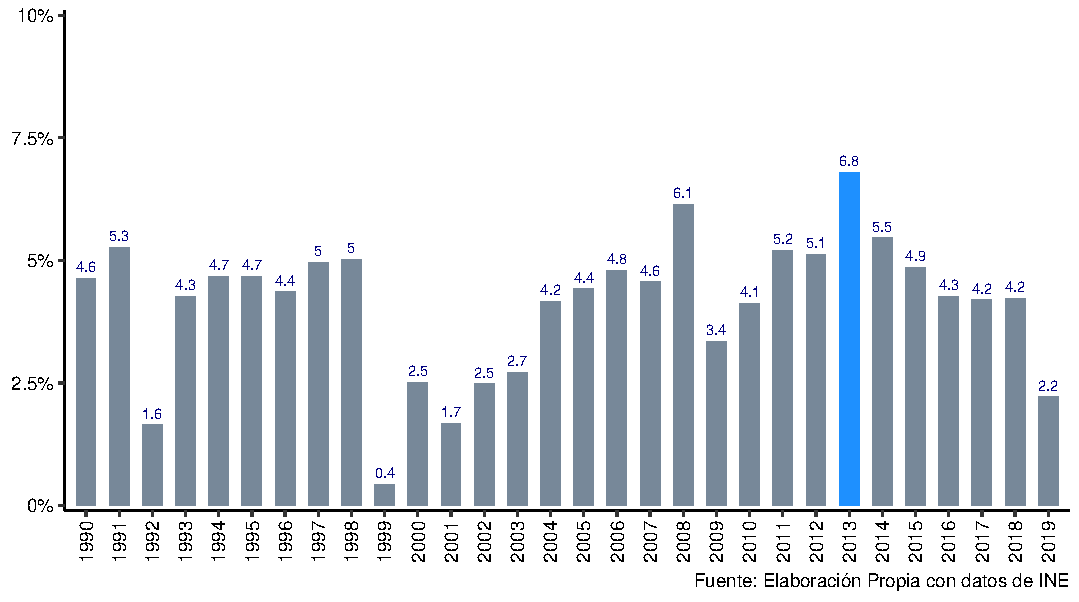
\includegraphics[scale=0.7]{Imagenes/pib_real_tasa.pdf}	
\end{figure}

Entre los aspectos clave de la inversión pública destacan, se justifica en que hay bienes o servicios que un privado no puede proveer de forma eficiente, es decir, generando beneficios. Por lo tanto, ante la ausencia de oferta, el Estado debe intervenir.

\section{La Inversión Publica}
\begin{figure}[!h]
	\centering
\caption{\label{fig:inversion}Ejecución de la Inversión Pública  1990-2019 \\ (En miles de dólares)}
	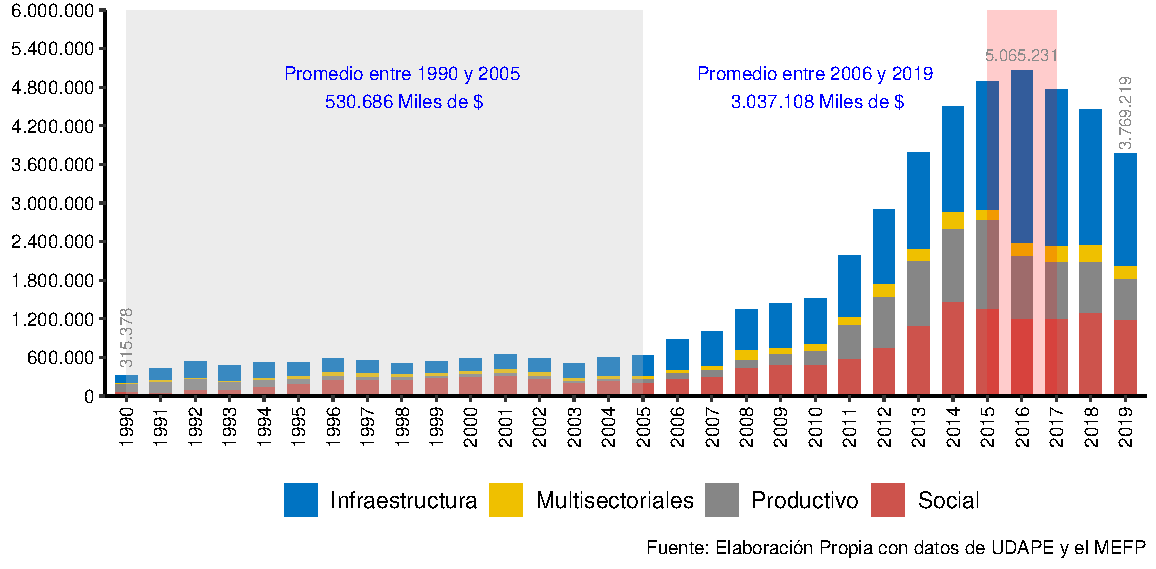
\includegraphics[scale=0.7]{Imagenes/inversion1.pdf}	
\end{figure}


\subsection{Infraestructura}
Un requisito indispensable para mantener el crecimiento de la economía en el largo plazo es contar con la infraestructura que requiere el sector productivo. Esto contribuirá a que
las empresas funcionen con mayor eficiencia y sean más productivas, toda vez que se reflejaría en una disminución de los costos de producción, con un beneficio directo para los consumidores.

Tener carreteras, puertos y ferrocarriles; líneas telefónicas; capacidad de generación, transmisión y distribución de energía eléctrica; una industria petrolera eficiente; presas y canales de irrigación, entre otras obras de infraestructura, es tarea del sector público e indispensable para elevar la competitividad y productividad de las empresas.

Sin embargo, para ello se requiere de una cantidad importante de recursos, que fueron escasos en años pasados dentro del Gobierno Federal, debido a los ajustes presupuestales que éste tuvo que realizar ante la debilidad de sus fuentes de ingresos y los objetivos de tener cuentas equilibradas. Aunque
estos ajustes contribuyeron al fortalecimiento de las finanzas públicas, generaron un rezago importante en materia de
inversión física. 


\section{Modelo}
La notación $AR(p)$ presenta un modelo autorregresivo de orden $p$. El modelo $AR(p)$ se define como:

$${\displaystyle X_{t}=c+\sum _{i=1}^{p}\varphi _{i}X_{t-i}+\varepsilon _{t}\,}$$

donde ${\displaystyle \varphi _{1},\ldots ,\varphi _{p}}{\displaystyle \varphi _{1},\ldots ,\varphi _{p}} $ son los parámetros del modelo, ${\displaystyle c} $es una constante, y ${\displaystyle \varepsilon _{t}}{\displaystyle \varepsilon _{t}}$ es ruido blanco. Esto se puede escribir de manera equivalente usando el operador de retroceso$B$ como

$$ {\displaystyle X_{t}=c+\sum _{i=1}^{p}\varphi _{i}B^{i}X_{t}+\varepsilon _{t}}$$

de manera que, moviendo el término sumatorio hacia el lado izquierdo y el uso de la notación polinómica, tenemos

$${\displaystyle \phi (B)X_{t}=c+\varepsilon _{t}}$$

Un modelo autorregresivo por lo tanto se puede ver como la salida de un todo- polo de impulso respuesta infinito filtro cuya entrada es ruido blanco.

Algunas limitaciones son necesarios en los valores de los parámetros de este modelo con el fin de que el modelo se mantiene estacionario en sentido amplio . Por ejemplo, los procesos $AR(1)$ con el modelo  no son estacionarias. Generalizando, para que un modelo $AR(p)$ sea estacionario en sentido amplio, las raíces del polinomio ${\displaystyle \textstyle z^{p}-\sum _{i=1}^{p}\varphi _{i}z^{p-i}}{\displaystyle \textstyle z^{p}-\sum _{i=1}^{p}\varphi _{i}z^{p-i}}$  debe estar dentro del círculo unitario, es decir, cada raíz ${\displaystyle z_{i}}{\displaystyle z_{i}} $ debe satisface.r

%\newpage


\section{Resultados}
como se observa en el Cuadro \ref{ref:resultados} los resultados 

\begin{table}[!h]
\begin{center}
\caption{\label{ref:resultados}Resultados de las Estimaciones por MCO}
\scalebox{0.85}{
\begin{tabular}{l c c c}
\hline
&&Variable dependiente&\\
& \multicolumn{3}{c}{\textit{Variable dependiente:}} \\
& \multicolumn{3}{c}{\textit{log(Pib\_Real)}} \\
& Model 1 & Model 2 & Model 3 \\
\hline
\hline
(Intercept)          & $12.45^{***}$ & $12.51^{***}$ & $12.32^{***}$ \\
                     & $(0.19)$      & $(0.15)$      & $(0.29)$      \\
log(Infraestructura) & $0.19^{***}$  & $0.18^{***}$  & $0.21^{***}$  \\
                     & $(0.05)$      & $(0.05)$      & $(0.03)$      \\
log(Social)          & $0.12^{**}$   & $0.11^{***}$  & $0.11^{**}$   \\
                     & $(0.03)$      & $(0.03)$      & $(0.03)$      \\
log(Productivo)      & $0.02$        & $0.02$        &               \\
                     & $(0.03)$      & $(0.03)$      &               \\
log(Multisectorial)  & $-0.01$       &               &               \\
                     & $(0.02)$      &               &               \\
\hline

R$^2$                & $0.97$        & $0.97$        & $0.91$        \\
Adj. R$^2$           & $0.97$        & $0.97$        & $0.91$        \\
Num. obs.            & $30$          & $30$          &            \\
rho                  & $$            & $$            & $0.55$        \\
number.interaction   & $$            & $$            & $8.00$        \\
dw.original          & $$            & $$            & $0.67$        \\
p.value.original     & $$            & $$            & $0.00$        \\
dw.transformed       & $$            & $$            & $1.58$        \\
p.value.transformed  & $$            & $$            & $0.04$        \\
nobs                 & $$            & $$            & $30$          \\
\hline
\hline
\multicolumn{4}{l}{\footnotesize{Nota: $^{***}p<0.001$; $^{**}p<0.01$; $^{*}p<0.05$}}
\end{tabular}
%\label{mco}
}
\end{center}
\end{table}  








\chapter{CONCLUSIÓN}
La influencia que Friedman ha ejercido en la profesión económica ha sido enorme y ello se refleja en la declaración de \cite{palley2014economia} en el sentido de que 
%% Bibliografia formato APA
\bibliographystyle{apalike}
\bibliography{biblioapa}


%% Anexo
\renewcommand{\appendixname}{ANEXO}
\renewcommand{\appendixtocname}{ANEXO}
\renewcommand{\appendixpagename}{ANEXO}

\appendix
\clearpage
\addappheadtotoc
\appendixpage
\chapter{Detalles Técnicos}
A veces, después de la investigación realizada a través de años de nuestro trabajo académico, contamos con mucho material que complementan nuestro artículo académico. Este material podría distraer o ser inapropiado en el cuerpo del manuscrito. 

\begin{center}
\begin{table}[!ht]
\centering
\caption{Datos de ...}

\begin{tabular}{ !{\vrule width 1pt}c!{\vrule width 1pt}c!{\vrule width 1pt}}
\noalign{\hrule height 1pt}
\cellcolor[gray]{0.9} \textbf{Año} &
\cellcolor[gray]{0.9} \textbf{Porcentaje}
\\ \noalign{\hrule height 1pt}
2000 & $0.29\%$
\\ \hline
2001 & $0.45\%$
\\ \hline
2002 & $0.68 \%$
\\ \hline
2003 & $1.01 \%$
\\ \hline
2004 & $1.47 \%$
\\ \hline
2005 & $5.48 \%$
\\ \noalign{\hrule height 1pt}
\end{tabular}
%\label{table:moneda}
\end{table}
\end{center}


\section{Correlación} 
\begin{figure}[!h]
	\centering
\caption{\label{fig:correlacion}Correlación de las Variables}
	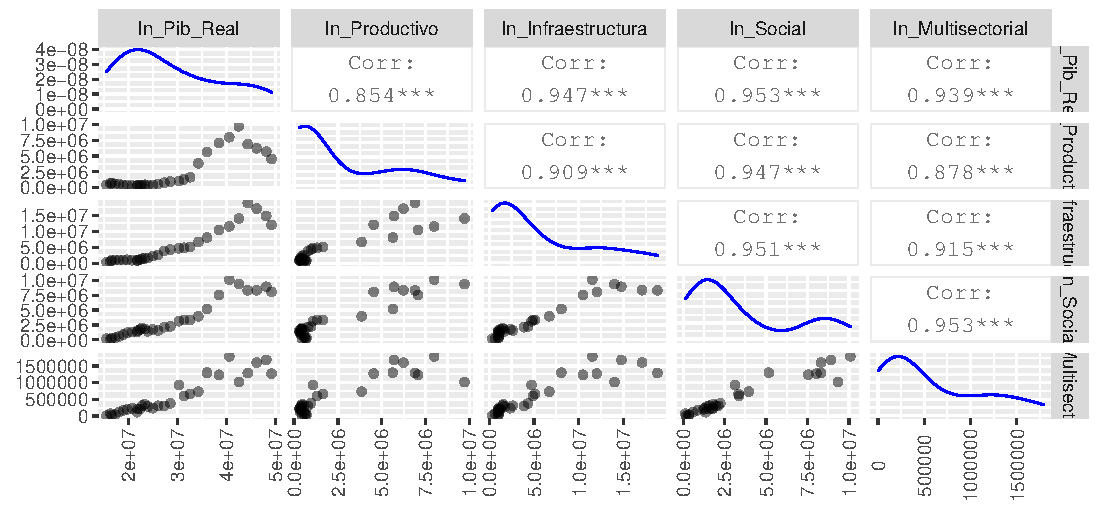
\includegraphics[scale=0.7]{Imagenes/correlacion1.pdf}	
\end{figure}

\chapter{Pruebas de Robustez}
En general, un apéndice es apropiado para materiales que son relativamente breves y que se presentan fácilmente en formato impreso. Algunos ejemplos de material adecuado para un apéndice son:

\begin{table}[!hbt]
\centering
\caption{ Como Realizar un Cuadro }
\begin{tabular}{|c|l|r|r|}
\hline N& Item& Precio& Cantidad\\
\hline \rowcolor{red}[0.9\tabcolsep]
\rule{0pt}{2.9ex}\noindent 1& A& 35& 140\\
\hline \rowcolor[gray]{0.7}[0.91\tabcolsep]
\rule{0pt}{2.7ex}\noindent 2& B& 55& 55\\
\hline \rowcolor{green}[0.91\tabcolsep]
\rule{0pt}{2.7ex}\noindent 3& C & 75& 75\\
\hline \multicolumn{3}{|r|}{Total}&
\cellcolor{blue} 270\\
\hline
\end{tabular}
\end{table}

\centering
\tcbox[left=0pt,right=0pt,top=0.5ex,bottom=0pt,boxsep=0pt,
toptitle=0.5ex,bottomtitle=0.5ex,title=Muestra de Tabla]{

\begin{tabular}[t]{rl}
Numero 1 & 100 \\
Numero 2 & 100 \\
Numero 3 & 150 \\
Sum & 350
\end{tabular}}

\end{document}
